\documentclass[10pt]{article}
\usepackage[pdftex]{graphicx}
\graphicspath{{./images/}}
\usepackage{amsmath,amssymb}
\usepackage{dirtytalk}
\usepackage{anyfontsize}
\usepackage{xcolor}
\usepackage{hyperref}
\usepackage{graphicx} 
\usepackage{placeins}
\hypersetup{
	colorlinks,
	linkcolor={red!50!black},
	citecolor={blue!50!black},
	urlcolor={blue!80!black}
}
\usepackage[skip=10pt plus1pt, indent=40pt]{parskip}
\usepackage{../common-styles/csagh}


\begin{document}
	\begin{opening}
		\title{Avance - PIA Investigación de Operaciones}
		\author[Universidad Autónoma de Nuevo León, San Nicolás de los Garza, aldo.hernandezt@uanl.edu.mx]{Aldo Hernández}
		\author[Universidad Autónoma de Nuevo León, San Nicolás de los Garza, abraham.lopezg@uanl.edu.mx]{Abraham López}
		
		\keywords{...}
		\begin{abstract}
            El Instituto Mexicano del Seguro Social es la entidad más popular y accesible para recibir atención médica a nivel nacional, sin embargo es debido a esta misma razón que es común que haya una gran cantidad de pacientes diarios en cada una de las unidades médicas, lo que alarga los tiempos de atención para todos los ciudadanos que requieren algún tipo de procedimiento médico. Este estudio busca encontrar un balance entre los tiempos de espera y los costos del hospital con el propósito de reducir los tiempos de espera promedio para los pacientes. Para lograr esto, se utilizará la teoría de colas para modelar un sistema particular en serie (o también conocido como tándem) y encontrar las medidas de desempeño para finalmente minimizar los costos y maximizar los consultorios; además, toda la información se obtendrá de fuentes públicas y accesibles para cualquier persona.
		\end{abstract}

		\keywords{colas, IMSS, python}
	\end{opening}
	
	\section{Introducción}
	La teoría de colas es una rama de las matemáticas que estudia el comportamiento de líneas de espera, buscando optimizar la eficiencia en los sistemas de servicio, en ella se analizan elementos como las tasas de llegada de usuarios, las tasas de servicio, el número de servidores y el orden de atención, entre otros factores. Este estudio se basa en un sistema de colas en serie (o tándem), donde distintos flujos de pacientes deben ser canalizados hacia un único punto de atención especializado, también conocido como un sistema de colas de múltiples entradas y una sola salida.
	
    Dentro del sistema de salud, la capacidad hospitalaria de una unidad médica es se enfoca en atender las necesidades de los pacientes a través de la organización \cite{MEDESK}, funcionamiento, gestión del personal, así como de la funcionalidad y disponibilidad de los recursos físicos y tecnológicos con los que debe contar un establecimiento de salud, calculados en función a sus características, dotación de recursos y demanda de atención. Algunos de los problemas más importantes que enfrentan estas unidades son su baja capacidad, las demoras y la programación inadecuada de sus recursos \cite{MEDESK} y podemos notar que estos tres problemas están relacionados, por ejemplo, una programación inadecuada de los pocos recursos y personal conlleva mayores tiempos de atención (e incluso servicio) por paciente.
    
    Es importante mencionar que la falta de recursos no suele ser un problema que dependa de la unidad completamente, sino que se ve influenciado por la fracción del presupuesto anual que destine el gobierno al sector de salud pública. Sin embargo, es común que la mala organización de dichos recursos acentúe esta falta de presupuesto más de lo que es; aquí es donde surge el problema de la optimización en la administración de estos recursos con el fin de lograr una mayor capacidad de servicio con un menor costo para la unidad.
    
    Por otra parte, además de la capacidad resolutiva de cada unidad, es fundamental diferenciar a las unidades en niveles de atención. Esto permite establecer un flujo de atención organizado y armonizado para las personas cuyas atenciones requieren transitar en tres diferentes niveles, con el fin de evitar la acumulación de pacientes en las distintas unidades de salud y lograr un menor tiempo de servicio.
    
    Para establecer de forma adecuada la vinculación de los tres niveles de atención, se requiere primeramente identificar el total de unidades médicas en operación dentro del sistema de salud y clasificarlas por nivel de atención de acuerdo a sus recursos, personal y cartera de servicios. Definiendo como objetivo de trabajo la generación de una metodología para realizar la clasificación por niveles de atención, se establece el siguiente proceso de trabajo, el cual se revisó y consensuó con todas las instituciones de salud en el marco del Comité Técnico especializado del Sector Salud (CTESS), así como con las Secretarías de Salud de los Estados.
    
    A pesar de este sistema de tres fases o niveles, la demanda de servicios de salud por unidad sigue siendo bastante alta, sobretodo en el primer nivel ya que no es necesario hacer cita previa para tener una consulta. Para evidenciar esto solo basta con acudir a cualquier unidad del seguro social para recibir una consulta, es tanta la reputación que tiene esta organización sobre la calidad de servicio y tiempo de espera que podría preguntarle a cualquier persona registrada en el seguro social si ha tenido alguna mala experiencia con estos temas. Es por esto que el IMSS ideó un sistema llamado UNIFILA a principios de 2017 para estos casos \cite{UNIFILA}, esta idea ofrece tres opciones para los pacientes sin cita:
    \begin{enumerate}
    	\item Programar el mismo día una cita con su médico familiar.
    	\item Programar una cita con su médico familiar la fecha más próxima.
    	\item Pasar al módulo UNIFILA para obtener una cita en los consultorios con espacios disponibles.
    \end{enumerate}
    
    Si bien esta implementación es bastante prometedora teóricamente, en la práctica resulta contraproducente ya que los testimonios de tiempos de espera siguen siendo bastante altos; esto podría ser debido a que si una gran sección de los pacientes ingresan a una clínica sin cita pues a final de cuentas todos tendrían que esperar a que se liberen espacios en los consultorios que estén ocupados por las personas que ya tienen cita.
    
    El problema que abordaremos se centra en el seguimiento de pacientes del primer nivel de atención hacia el tercer nivel dentro del sistema de salud del IMSS (Instituto Mexicano del Seguro Social), para ello, utilizaremos dos conjuntos de datos de consultas: uno sobre unidades de primer nivel y otro sobre las de tercer nivel. Estos datos contienen información de atenciones médicas realizadas en septiembre de 2017 mediante la encuesta EnSat \cite{ensat2017} llevada a cabo al menos una vez al año por el IMSS.
    
    Se eligieron los resultados de este año ya que es uno de los conjuntos con más registros de información y también debido a que a partir de 2019 se sustituyó esta encuesta por otra llamada EnCal; si bien esta encuesta está mejor estructurada, también omite muchas preguntas relevantes para este estudio.
    
    El principal enfoque para el estudio serán los tiempos de espera basándonos en la siguiente pregunta: ¿por qué el paciente promedio tiene que esperar tantos días para recibir la atención médica que necesita?

	\section{Contexto}
	En el sistema de salud del IMSS, los pacientes deben ser atendidos inicialmente en unidades médicas de primer nivel, éstas otorgan exclusivamente atención ambulatoria, que puede ser general o especializada; en dichas unidades inicia el primer contacto con los pacientes fungiendo como principales vehículos para realizar acciones de prevención y promoción a la salud, así como la detección temprana y seguimiento de enfermedades, son la vía de entrada al sistema de atención y, en caso necesario, son referidos a hospitales de tercer nivel, que son las que otorgan atención médica hospitalaria para la atención de padecimientos de alta especialidad y de urgencias.
	
    Este proyecto se centrará específicamente en la Unidad Médica Familiar No. 28 (UMF 28) de Monterrey, Nuevo León, como punto de primer nivel, y en el Hospital de Especialidades No. 25 de Monterrey como punto de tercer nivel, ambos centros de atención se encuentran geográficamente cercanos, lo cual facilita el análisis de la transferencia de pacientes entre ellos.
    
    \begin{figure}[h]
		\centering
		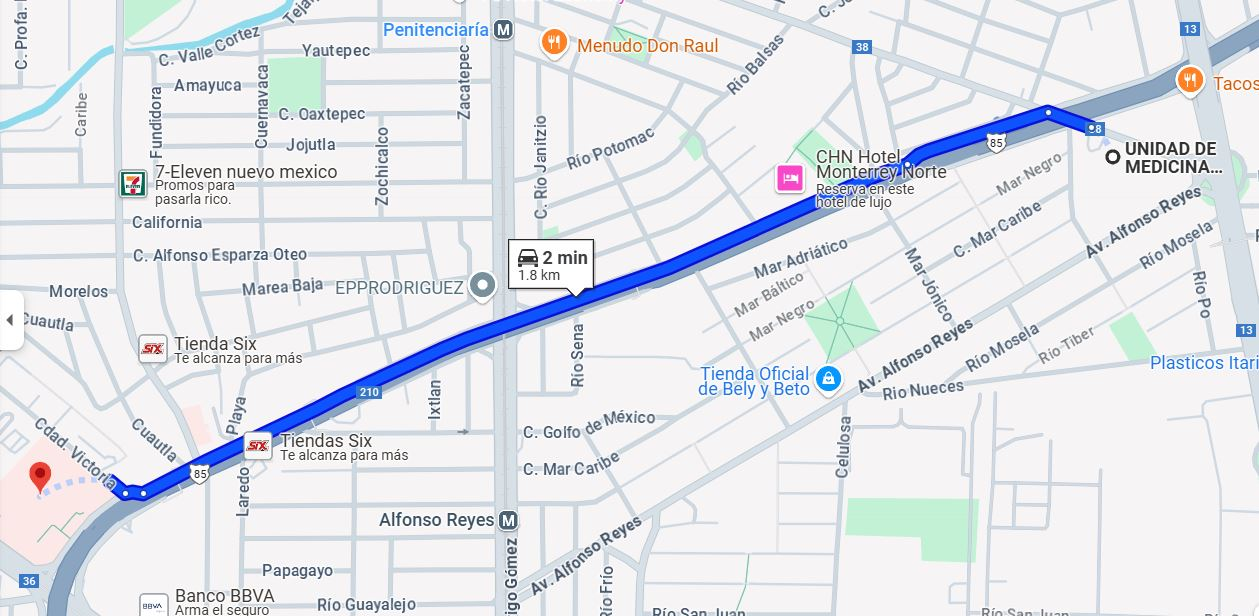
\includegraphics[width=90mm]{./images/mapa.jpg}
		\caption{Distancia entre los dos centros.}
	\end{figure}
	\FloatBarrier

    Antes de proceder con el análisis, será necesario realizar un proceso de limpieza de los conjuntos de datos, pues decidimos que no haremos distinciones en cuestión de edades, sexo o tipo de paciente aunque existan columnas que nos hablen sobre estas características de la persona, por lo que elminaremos los registros no necesarios y seleccionaremos solo aquellos campos relevantes para el propósito de este estudio como lo son los tiempos de espera y el servicio otorgado.
    
    El flujo de atención será modelado en tres etapas:

    \begin{enumerate}
        \item \textbf{Primera etapa (UMF 28)}: Los pacientes llegan a consulta general, donde son atendidos por múltiples médicos de primer contacto. Esta situación se modela mediante un sistema de colas \textbf{M/M/s}.
        
        \item \textbf{Segunda etapa (Proceso de referencia)}: Los pacientes que requieren atención especializada son referidos a través de un proceso administrativo, modelado como un sistema de colas \textbf{M/M/1}.
        
        \item \textbf{Tercera etapa (Hospital 25)}: Los pacientes son atendidos por múltiples especialistas de tercer nivel, modelado nuevamente como un sistema de colas \textbf{M/M/s}.
    \end{enumerate}

    \begin{figure}[h]
		\centering
		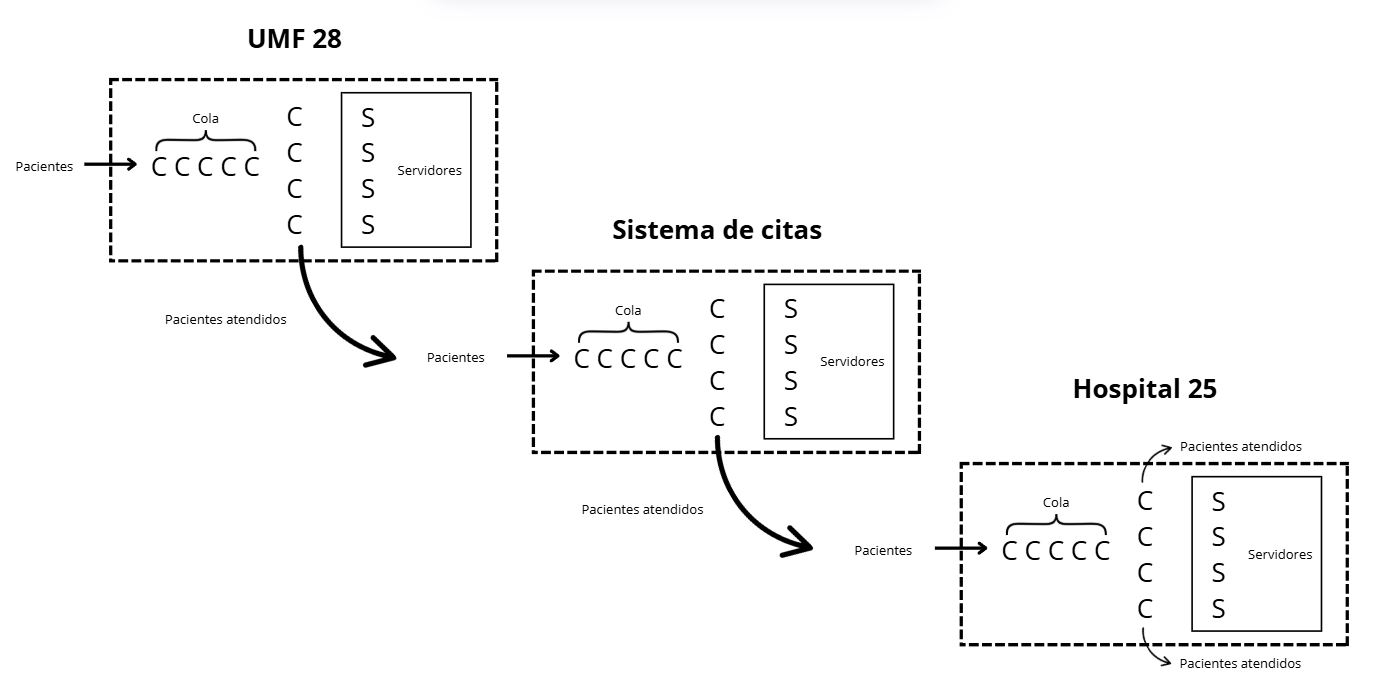
\includegraphics[width=130mm]{./images/sistema.jpg}
		\caption{Modelo.}
	\end{figure}

    Una vez que el paciente recibe la atención especializada, existen tres posibles desenlaces, el paciente se cura y no requiere más atención (salida del sistema), el paciente requiere seguimiento y debe regresar al hospital o el paciente abandona el tratamiento por voluntad propia. Cabe aclarar que este estudio se concentrará en el caso de la salida del sistema, puesto que asumimos un caso ideal en el que el paciente busca mejorarse y además no tiene múltiples consultas ya que eso agrandaría el flujo del sistema a estudiar.

    \section{Datos y problema}
    Después de realizar una limpieza básica para eliminar datos innecesarios y registros vacíos, filtramos únicamente los datos correspondientes a las unidades médicas mencionadas. Además, es importante mencionar que se asumió una distribución de probabilidad exponencial para cada una de las colas tanto para los tiempos entre llegadas como los tiempos de servicio. En las siguientes subsecciones se explicarán los procesos llevados a cabo en cada una de las colas. \par
    El caso general a estudiar se detallará a continuación. Una persona con seguro social en el IMSS comienza a tener síntomas de alguna enfermedad, por lo que acude a la Unidad de Medicina Familiar 28 para una consulta de primer nivel habiendo hecho cita previa para el mismo día. Al llegar al centro de salud, tiene que esperar en una sala mientras se libera un consultorio para que lo puedan atender y cuando finalmente lo revisa el doctor en turno, resulta que su caso requiere de un chequeo realizado por un especialista, por lo que es referenciado al Hospital de Especialidades 25. Sin embargo, el paciente tiene que sacar una cita previa para poder ser recibido en el hospital para consulta, por lo que al tramitarla la espera es de varios días. Finalmente, acude el día de su cita al centro de salud donde todavía tiene que volver a esperar en una sala para que lo pasen a un consultorio, una vez saliendo del chequeo, el paciente se cura y se le da de alta. \par
    Cabe mencionar que estos valores son aproximados ya que no es información que suela capturarse o hacerse pública, por lo que solo podemos hacer estimaciones en base a las fuentes de información referenciadas. \par
    
    \subsection{Primera cola (M/M/$s_{1}$)}
    Los pacientes se generan en una fuente de entrada finita lo suficientemente grande como para no preocuparnos por la población debido a que este tipo de unidades casi nunca se saturan de pacientes, entonces se tomará como una fuente ilimitada. Además, se asumirá una distribución Poisson para las llegadas de pacientes bajo el supuesto de que llegan aleatoriamente con una cierta tasa media fija, por lo que el tiempo entre llegadas sigue una distribución exponencial. Se ignorarán los casos en los que los pacientes se rehúsan a entrar al sistema (debido a que en un caso ideal su salud debería ser la prioridad) junto con la distinción de grupos entre los pacientes (por edad, enfermedad, entre otros) de tal manera que para cálculos generales se considerará el conjunto completo mientras que para las medidas de desempeño solo se tomarán en cuenta datos de pacientes del caso general del sistema de colas. \par
    La cola se considerará infinita a pesar de tener alguna cota superior ya que tomarla en cuenta complicaría el análisis. Esta cola tendrá una disciplina FIFO, de manera que los pacientes serán atendidos a como vayan llegando a la sala de espera. \par
    La estación de servicio contiene $s_{1}$ servidores activos la jornada completa de 12 horas cuyos tiempos de servicio siguen una distribución exponencial para todos los pacientes. Nótese que $s_{1}$ todavía no está definida, por lo que estudiaremos distintos valores para dicha variable a fin de encontrar un balance entre costos y tiempos de espera. \par
    Finalmente, medimos los siguientes parámetros para esta cola: \par
    
    \begin{equation*}
    	\left\{
    		\begin{array}{@{}l@{}}
	    		\frac{1}{\lambda} = \frac{720 \text{ minutos}}{160 \text{ pacientes}} = 4.5 \text{ minutos por paciente,} \\
	    		\lambda = 0.22 \text{ pacientes por minuto,} \\
	    		\frac{1}{\mu} = 15 \text{ minutos por paciente,} \\
	    		\mu = 0.066 \text{ pacientes por minuto} \\
	    		W_{q} = 18.64 \text{ minutos,} \\
	    		W = 33.64 \text{ minutos,} \\
	    		\left\lceil L \right\rceil = 8 \text{ pacientes,} \\
	    		\left\lfloor L_{q} \right\rfloor = 4 \text{ pacientes}
    		\end{array}
   		\right.\,.
    \end{equation*}
    
    Para obtener esta información bastó con revisar información en internet \cite{IMSS2022} para obtener un aproximado de los pacientes diarios en promedio por unidad de medicina familiar a nivel nacional y asumir un tiempo de servicio de 15 minutos. Además, se consultó el conjunto de datos para obtener el tiempo de espera promedio en la cola mediante una media de datos agrupados según los datos que se muestran en la figura \ref{fig:frec_espera_umf28}. Para los valores de $L$ y $L_{q}$ se optó por usar la función piso o techo según si los decimales eran despreciables o no, respectivamente, ya que tienen que ser números enteros.
    
    \begin{figure}[h]
    	\centering
    	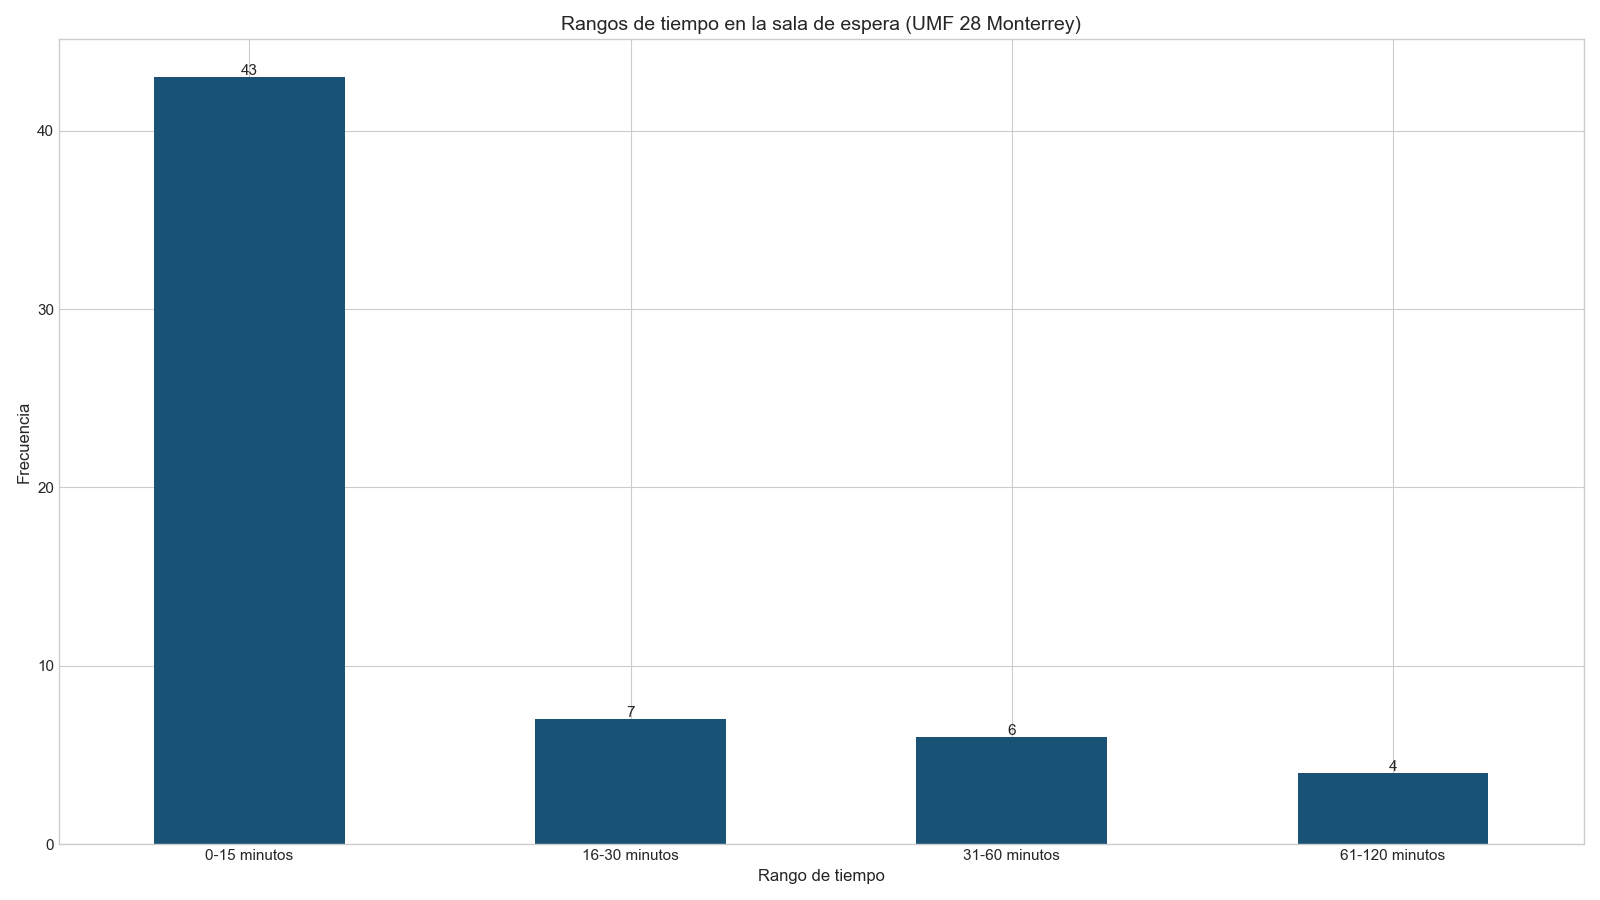
\includegraphics[width=130mm]{./images/rangos-tiempo-espera-umf28.png}
    	\caption{Gráfica de frecuencias para los tiempos de espera en la UMF 28.}
    	\label{fig:frec_espera_umf28}
    \end{figure}
    
    \newpage
    
    \subsection{Segunda cola (M/M/1)}
    Los pacientes se generan en una fuente de entrada finita lo suficientemente grande como para no preocuparnos por la población debido a que en el flujo del sistema estos pacientes son aquellos que al salir de su consulta en alguna unidad de primer nivel de atención requieren una cita posterior en una unidad de tercer nivel, entonces se tomará como una fuente ilimitada. Además, se asumirá una distribución Poisson para las llegadas de pacientes bajo el supuesto de que llegan aleatoriamente con una cierta tasa media fija, por lo que el tiempo entre llegadas sigue una distribución exponencial. Se ignorarán los casos en los que los pacientes se rehúsan a entrar al sistema (debido a que en un caso ideal su salud debería ser la prioridad) junto con la distinción de grupos entre los pacientes (por edad, enfermedad, entre otros). \par
    La cola se considerará infinita a pesar de tener alguna cota superior ya que tomarla en cuenta complicaría el análisis. Esta cola tendrá una disciplina FIFO, de manera que los pacientes serán atendidos a como vayan solicitando su cita en el IMSS. \par
    La estación de servicio contiene un único servidor activo (el "sistema") las 24 horas del día y sus tiempos de servicio siguen una distribución exponencial para todos los pacientes. \par
    Finalmente, medimos los siguientes parámetros para esta cola:
    
    \newpage
    
    \begin{equation*}
    	\left\{
    	\begin{array}{@{}l@{}}
    		\frac{1}{\lambda} = \frac{1 \text{ día}}{200 \text{ pacientes}} = 0.005 \text{ días por paciente,} \\
    		\lambda = 200 \text{ pacientes por día,} \\
    		\frac{1}{\mu} = 1 \text{ día por paciente,} \\
    		\mu = 1 \text{ paciente por día} \\
    		W_{q} = 16.52 \text{ días,} \\
    		W = 17.52 \text{ días,} \\
    		L = 3504 \text{ pacientes,} \\
    		L_{q} = 3304 \text{ pacientes}
    	\end{array}
    	\right.\,.
    \end{equation*}
    
    Para obtener esta información se consultó el conjunto de datos para obtener el tiempo de espera promedio en la cola mediante una media de datos agrupados según los datos que se muestran en la figura \ref{fig:frec_espera_cita}.
    
    \begin{figure}[h]
    	\centering
    	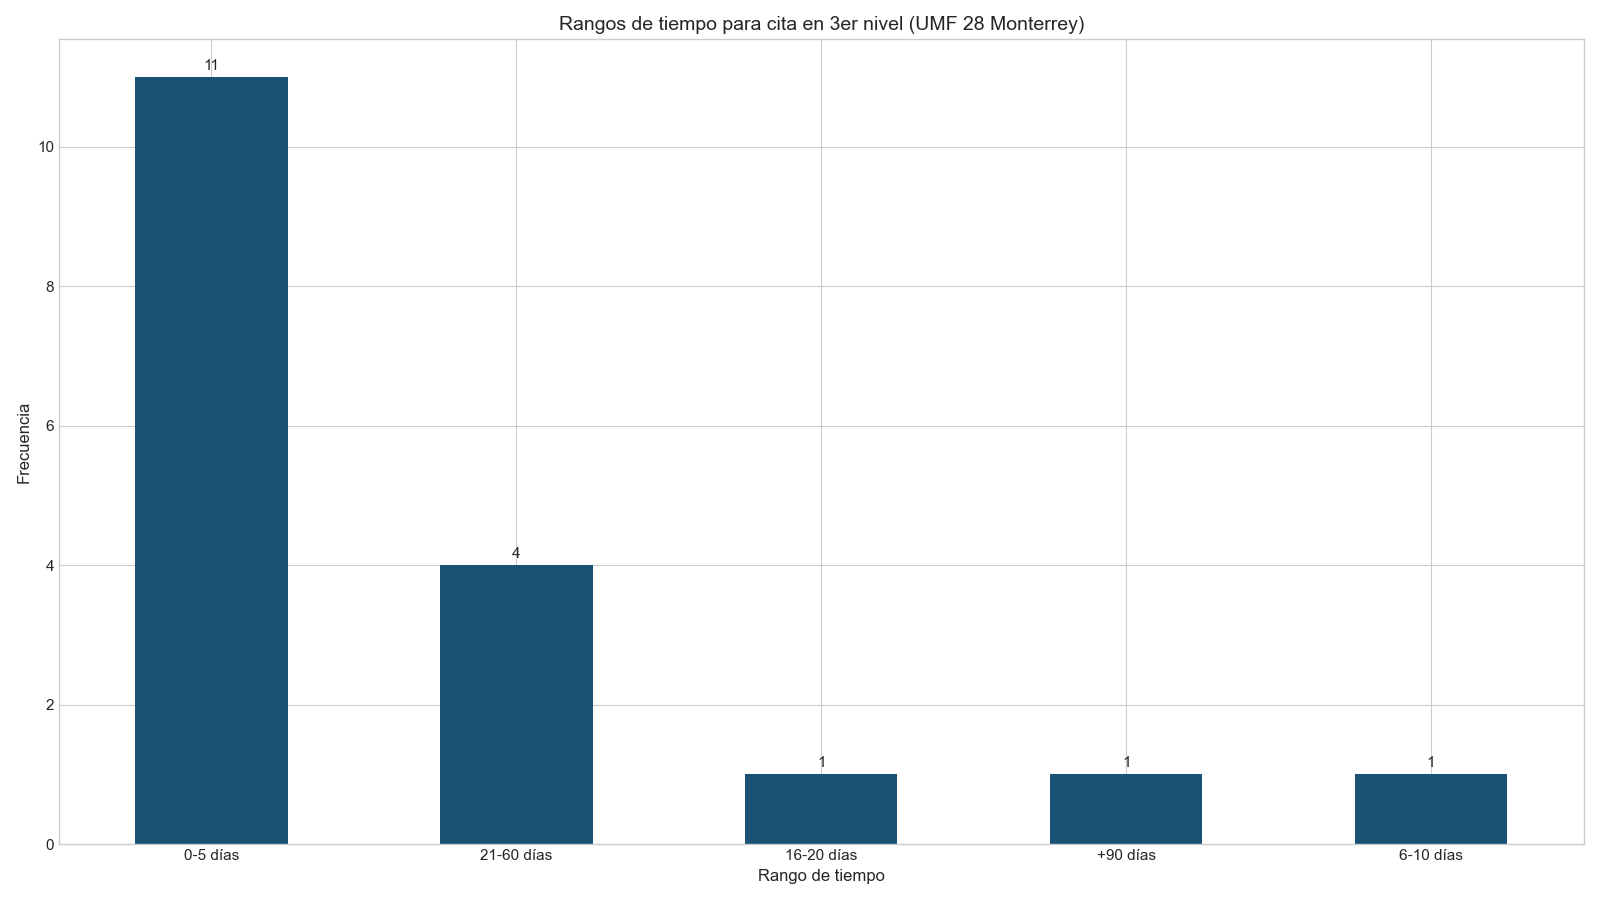
\includegraphics[width=130mm]{./images/rangos-tiempo-3-umf28.png}
    	\caption{Gráfica de frecuencias para los tiempos de espera en el sistema de citas.}
    	\label{fig:frec_espera_cita}
    \end{figure}
    
    \subsection{Tercera cola (M/M/$s_{2}$)}
    Los pacientes se generan en una fuente de entrada finita lo suficientemente grande como para no preocuparnos por la población debido a que este tipo de unidades de alta especialidad casi nunca se saturan de pacientes, entonces se tomará como una fuente ilimitada. Además, se asumirá una distribución Poisson para las llegadas de pacientes bajo el supuesto de que llegan aleatoriamente con una cierta tasa media fija dictada por el sistema de citas, por lo que el tiempo entre llegadas sigue una distribución exponencial. Se ignorarán los casos en los que los pacientes se rehúsan a entrar al sistema (debido a que en un caso ideal su salud debería ser la prioridad) junto con la distinción de grupos entre los pacientes (por edad, enfermedad, entre otros). \par
    La cola se considerará infinita a pesar de tener alguna cota superior ya que tomarla en cuenta complicaría el análisis. Esta cola tendrá una disciplina FIFO, de manera que los pacientes serán atendidos a como vayan llegando a la sala de espera. \par
    La estación de servicio contiene $s_{2}$ servidores activos la jornada completa de 12 horas cuyos tiempos de servicio siguen una distribución exponencial para todos los pacientes. Nótese que $s_{2}$ todavía no está definida, por lo que estudiaremos distintos valores para dicha variable a fin de encontrar un balance entre costos y tiempos de espera. \par
    Finalmente, medimos los siguientes parámetros para esta cola: \par
    
    \begin{equation*}
    	\left\{
    	\begin{array}{@{}l@{}}
    		\frac{1}{\lambda} = \frac{720 \text{ minutos}}{82 \text{ pacientes}} = 8.78 \text{ minutos por paciente,} \\
    		\lambda = 0.11 \text{ pacientes por minuto,} \\
    		\frac{1}{\mu} = 30 \text{ minutos por paciente,} \\
    		\mu = 0.033 \text{ pacientes por minuto} \\
    		W_{q} = 18.51 \text{ minutos,} \\
    		W = 48.51 \text{ minutos,} \\
    		\left\lceil L \right\rceil = 6 \text{ pacientes,} \\
    		\left\lfloor L_{q} \right\rfloor = 2 \text{ pacientes}
    	\end{array}
    	\right.\,.
    \end{equation*}
    
    Para obtener esta información bastó con revisar el conjunto de datos para obtener dos cosas principalmente: el tiempo de espera promedio en la cola mediante una media de datos agrupados según los datos que se muestran en la figura \ref{fig:frec_espera_hes25} y una cantidad aproximada de pacientes diarios que acuden con un especialista, esta última información se obtuvo a partir de que en los registros se cuentan solo con 32 casos de consulta con especialista de los 74 totales para esta unidad y si suponemos una cantidad de 190 pacientes diarios en todo el hospital, se obtienen los 82 pacientes diarios en promedio que acuden con un especialista. Por otro lado, para los valores de $L$ y $L_{q}$ se optó por usar la función piso o techo según si los decimales eran despreciables o no, respectivamente, ya que tienen que ser números enteros.
    
    \begin{figure}[h]
    	\centering
    	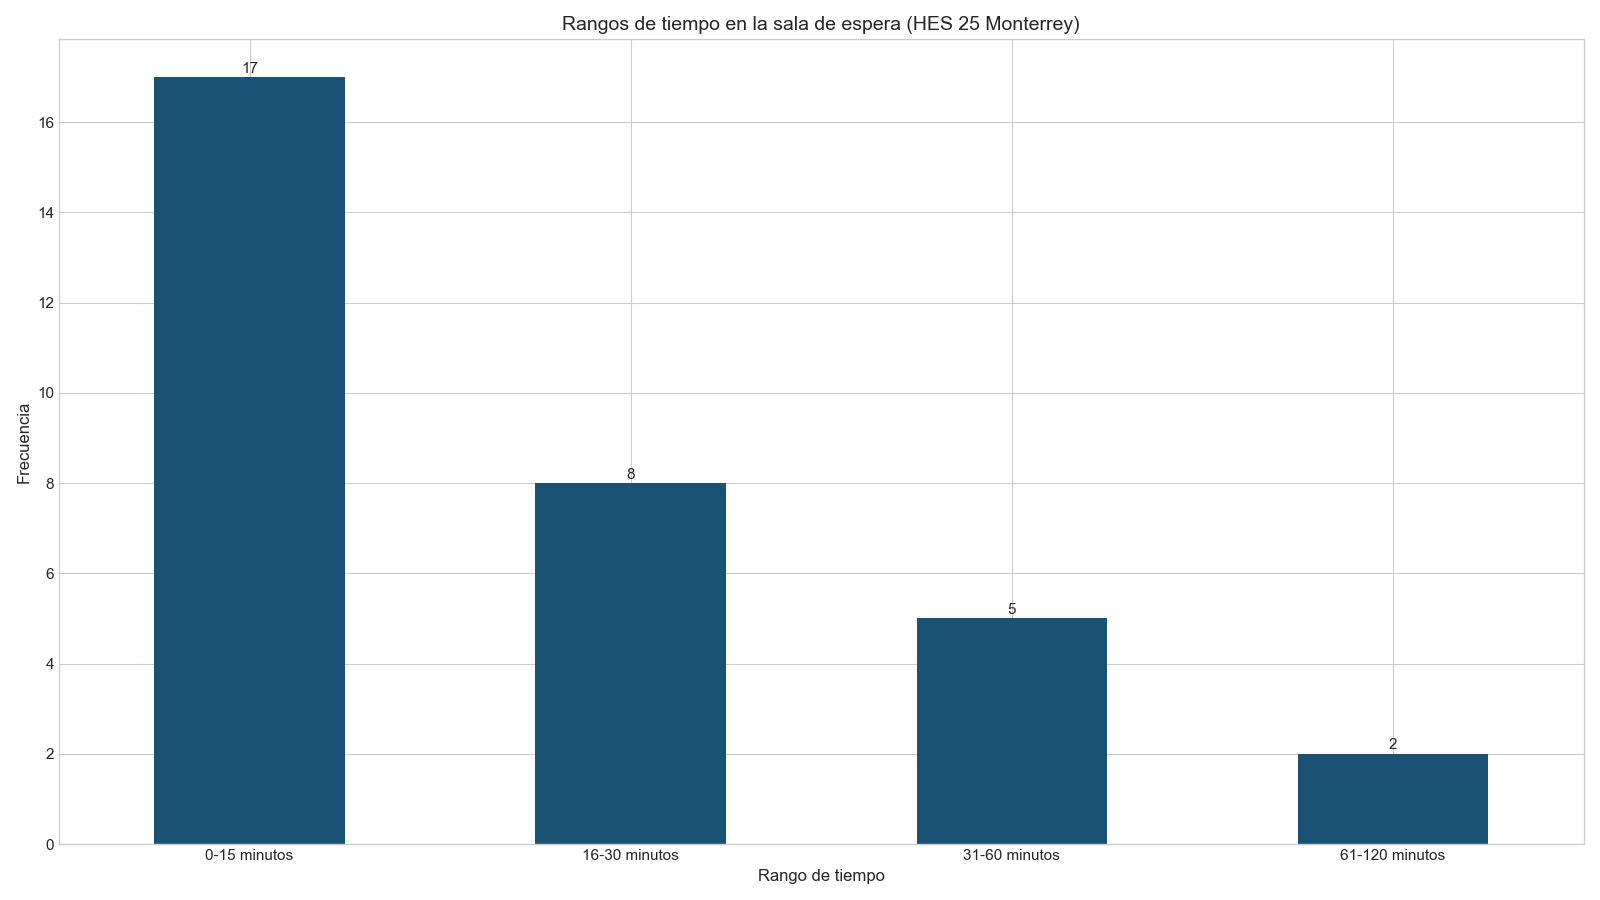
\includegraphics[width=130mm]{./images/rangos-tiempo-espera-hes25.png}
    	\caption{Gráfica de frecuencias para los tiempos de espera en el HES 25.}
    	\label{fig:frec_espera_hes25}
    \end{figure}
    
    \newpage
    
    \bibliographystyle{../common-styles/cs-agh}
    \bibliography{pia-bibliografia}

\end{document}